\documentclass[10pt,compress,mathserif]{beamer}
\usetheme{Berkeley}

\usepackage{amsmath,minibox,amssymb,amsfonts,amsthm,graphicx,color,multirow,array,tikz,hyperref}
\usetikzlibrary{arrows,snakes,backgrounds,patterns,matrix,shapes,fit,calc,shadows, positioning}

\setbeamertemplate{navigation symbols}{} % Remove navigation symbols
\setbeamerfont{caption}{size=\footnotesize}

\title[]{Control Systems Project}
\author[]{Syed Fahd Ali\\ Section C, DCSE\\ Enrollment Number: 21PWCSE1992}
\date{January 8, 2024}

\begin{document}

\begin{frame}    \titlepage \end{frame}

% First Slide
\section{Problem Statement}
\begin{frame}{Problem Statement}
Consider the following tasks for the inverted pendulum system:
\begin{itemize}
    \item Check the stability of the system using all known methods.
    \item Simulate the unstable system and show that its response is unstable.
    \item Compute the controllability and observability of the system. If the system is controllable, place the controller poles at \((-4, -3, -8, -5)\) and observer poles faster than the controller poles.
    \item Simulate the stable system and design a PID controller.
    \item Compute the steady-state errors before and after designing controllers.
\end{itemize}
\end{frame}

% Second Slide
\section{State-space Representation}
\begin{frame}{State-space Representation}
The state-space representation of the system is given by:
\[ \dot{x} = Ax + Bu, \quad y = Cx + Du \]
Where:
\[
A = \begin{bmatrix}
0 & 1 & 0 & 0 \\
0 & -0.818 & 2.6727 & 0 \\
0 & 0 & 0 & 1 \\
0 & -0.4545 & 31.1818 & 0
\end{bmatrix}, \quad
B = \begin{bmatrix} 0 \\ 1.8182 \\ 0 \\ 4.5455 \end{bmatrix}
\]
\[
C = \begin{bmatrix} 1 & 0 & 0 & 0 \end{bmatrix}, \quad D = 0
\]
\end{frame}

% Stability Analysis
\section{Stability Analysis}
\begin{frame}{Stability Analysis}
The eigenvalues of the system matrix \(A\) are:
\[ \lambda = \{0, 5.5670, -5.6067, -0.7783\} \]
The poles of the transfer function are:
\[ \text{Poles} = \{0, 5.5670, -5.6067, -0.7783\} \]
Since one eigenvalue and one pole have positive real parts, the system is unstable in open-loop configuration.
\end{frame}

\begin{frame}{Step Response of the System (Unstable)}
\begin{figure}[h!]
    \centering
    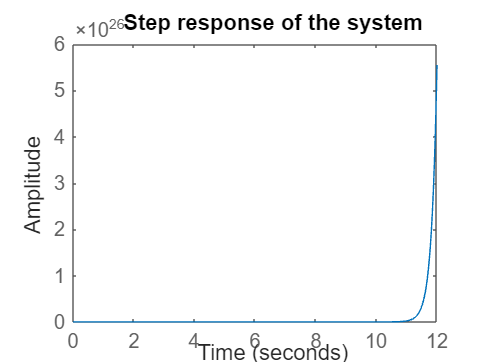
\includegraphics[scale=0.5]{step.png}
    \caption{Step Response of the System}
\end{figure}
\end{frame}

% Controllability and Observability
\section{Controllability and Observability}
\begin{frame}{Controllability and Observability}
The controllability and observability matrices have full rank, confirming that the system is controllable and observable.
\begin{figure}[h!]
    \centering
    \begin{minipage}{0.45\textwidth}
        \centering
        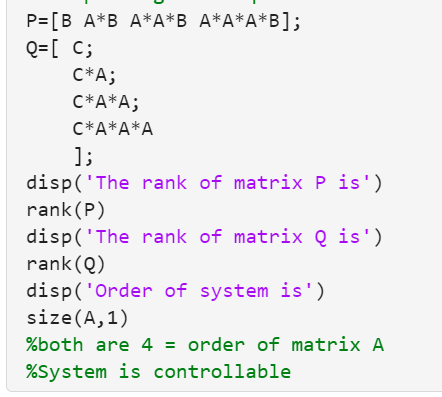
\includegraphics[width=\textwidth]{rank.png}
        \caption{Code for Controllability and Observability}
    \end{minipage}
    \hfill
    \begin{minipage}{0.45\textwidth}
        \centering
        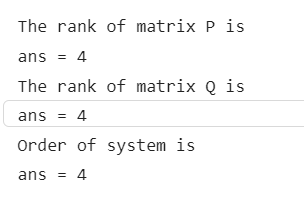
\includegraphics[width=\textwidth]{rank_output.png}
        \caption{Output of Controllability and Observability}
    \end{minipage}
\end{figure}
\end{frame}

% Controller Design
\section{Controller Design}
\begin{frame}{State-Feedback and Observer Design}
\textbf{State-Feedback Controller (SFC):}
\[ K = \begin{bmatrix} -10.7754 & -7.8698 & 37.9423 & 7.3679 \end{bmatrix} \]
\textbf{Observer Feedback Controller (OFC):}
\[ L = \begin{bmatrix} 0.0212 \\ 0.1849 \\ 0.4650 \\ 2.5916 \end{bmatrix} \]
Closed-loop system matrices:
\[ A_{clp} = A - BK, \quad A_{clp2} = A - LC \]
\end{frame}

\begin{frame}{Controller Design Simulation}
\begin{figure}[h!]
    \centering
    \begin{minipage}{0.45\textwidth}
        \centering
        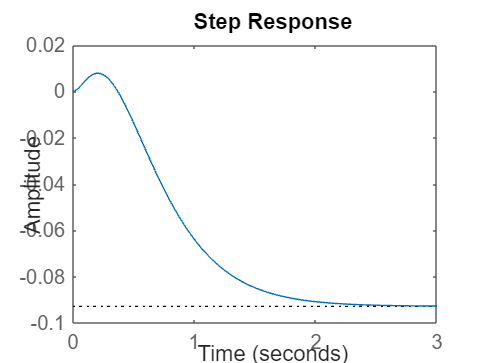
\includegraphics[width=\textwidth]{state_feedback.png}
        \caption{Response for State Feedback Controller}
    \end{minipage}
    \hfill
    \begin{minipage}{0.45\textwidth}
        \centering
        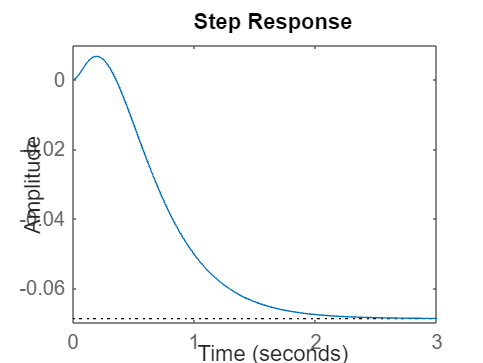
\includegraphics[width=\textwidth]{observer_feedback.png}
        \caption{Response for Observer Feedback Controller}
    \end{minipage}
\end{figure}
\end{frame}

% PID Controller Design
\section{PID Controller Design}
\begin{frame}{PID Controller Design}
The PID controller parameters are:
\[ K_p = -0.0552, \quad K_i = -0.000684, \quad K_d = -1.11 \]
The closed-loop system transfer function is:
\[
\text{sys}_{\text{now}} = \frac{-2.024s^4 - 0.1003s^3 + 49.6s^2 + 2.458s + 0.03046}{s^5 - 1.206s^4 - 31.28s^3 + 25.3s^2 + 2.458s + 0.03046}
\]
\end{frame}

\begin{frame}{Step Response with PID Controller}
\begin{figure}[H]
    \centering
    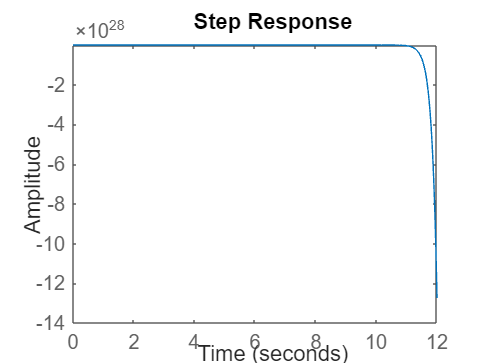
\includegraphics[scale=0.5]{PID.png}
    \caption{Response for PID Controller}
\end{figure}
\end{frame}

% Simulation Results
\begin{frame}{Steady-State Errors and Results}
    DC gains before and after controllers for Step :
    \[
    \begin{aligned}
    &\text{DC gain (Open-loop)} = \infty, \\
    &\text{DC gain (SFC)} = -0.0928, \\
    &\text{DC gain (OFC)} = -0.0687, \\
    &\text{DC gain (PID)} = 1
    \end{aligned}
    \]
    Steady-state errors for Step:
    \[
    \begin{aligned}
    &\text{Error (Open-loop)} = 0, \\
    &\text{Error (SFC)} = 1.1023, \\
    &\text{Error (OFC)} = 1.0738, \\
    &\text{Error (PID)} = 0.5
    \end{aligned}
    \]
\end{frame}
    
\begin{frame}{Simulation Results in Simulink}
\begin{figure}[h!]
    \centering
    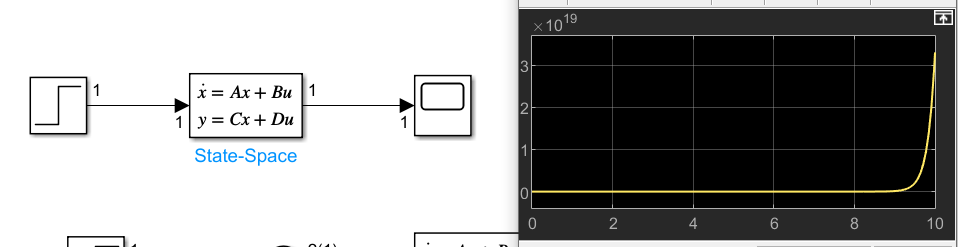
\includegraphics[scale=0.5]{simulink_system_response.png}
    \caption{Simulink System Response}
\end{figure}
\end{frame}

\begin{frame}{Simulink Controllers}
\begin{figure}[h!]
    \centering
    \begin{minipage}{0.6\textwidth}
        \centering
        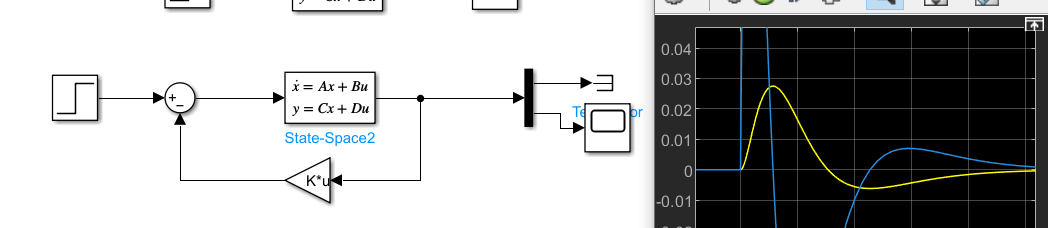
\includegraphics[width=\textwidth]{sl_sfc.png}
        \caption{Simulink State Feedback Controller}
    \end{minipage}
    \hfill
    \begin{minipage}{0.6\textwidth}
        \centering
        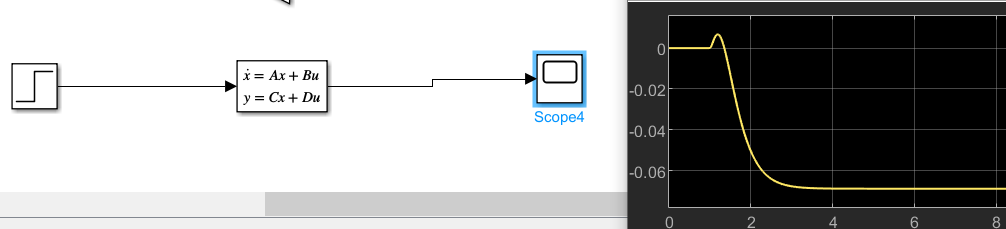
\includegraphics[width=\textwidth]{sl_obs.png}
        \caption{Simulink Observer Feedback Controller}
    \end{minipage}
\end{figure}
\begin{figure}[h!]
    \centering
    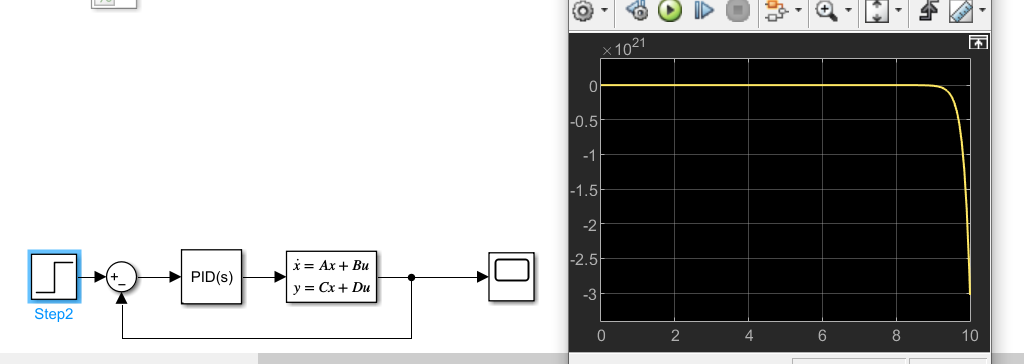
\includegraphics[scale=0.4]{sl_PID.png}
    \caption{Simulink PID Feedback Controller}
\end{figure}
\end{frame}

\end{document}
